% SOURCE: base_noise_swamping_20260726.json fields per_cell.*.{noise_to_signal_ratio,flat_rank_survival,base_quant_noise_mean_abs}.
% !TEX encoding = UTF-8 Unicode
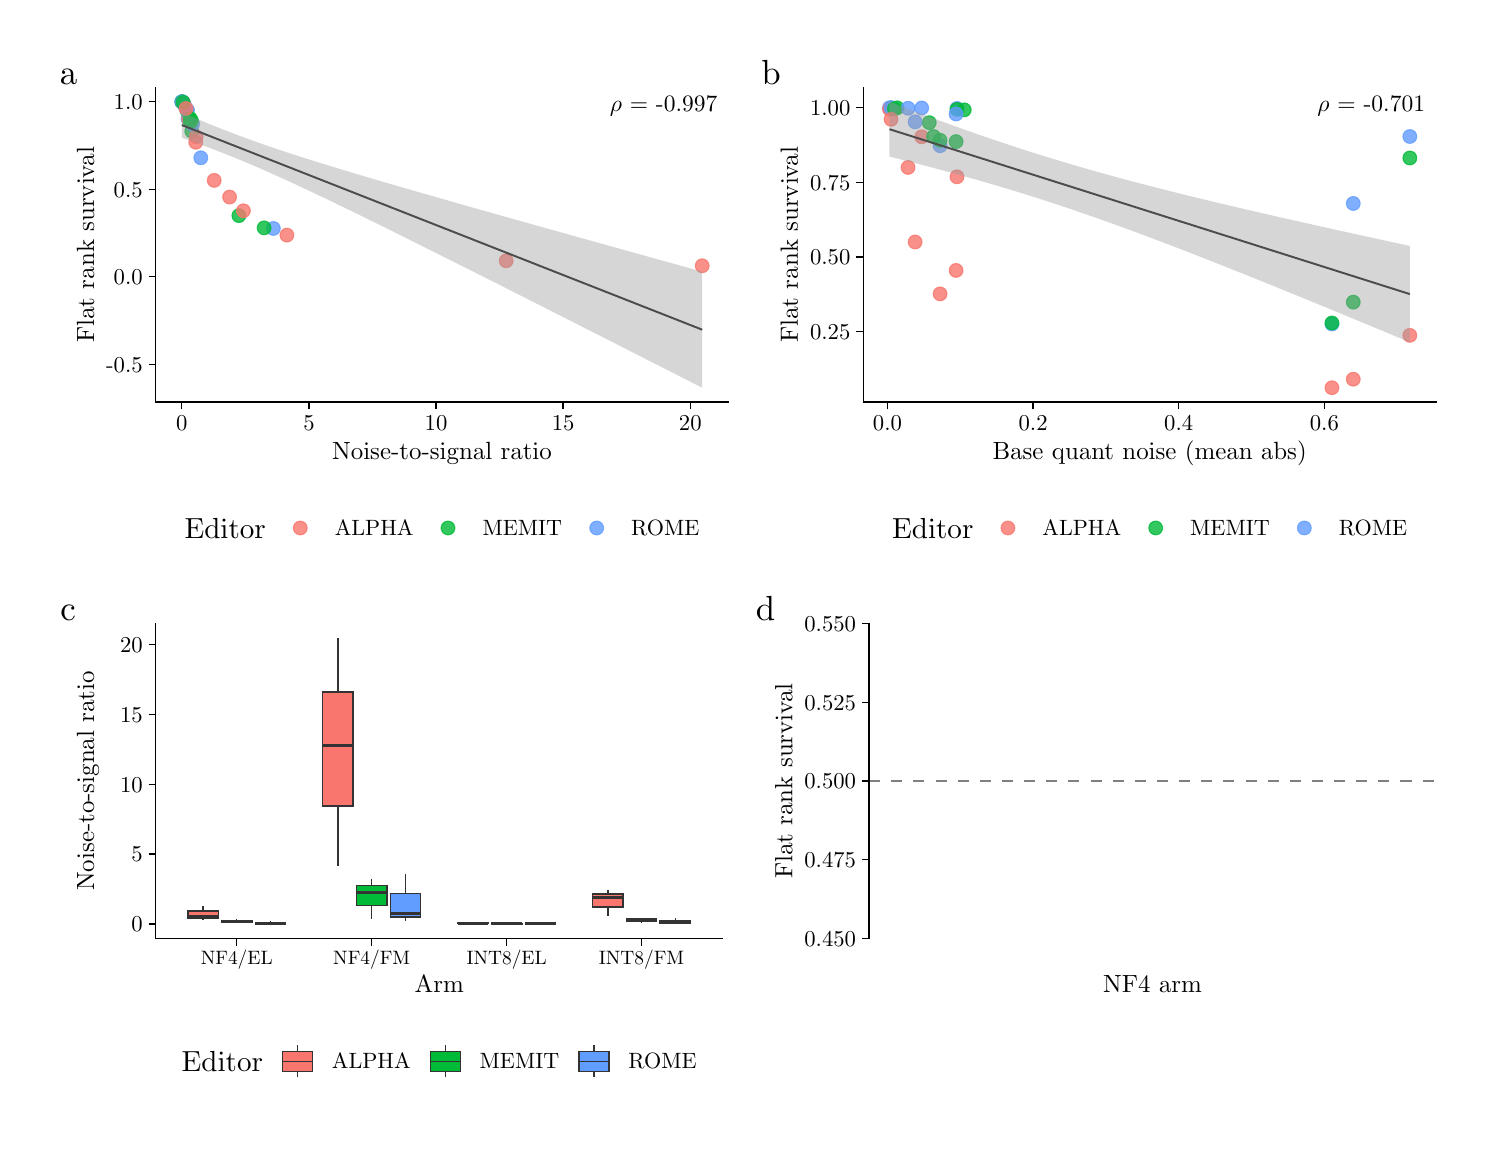
\begin{tikzpicture}[x=1pt,y=1pt]
\definecolor{fillColor}{RGB}{255,255,255}
\path[use as bounding box,fill=fillColor,fill opacity=0.00] (0,0) rectangle (520.34,397.48);
\begin{scope}
\path[clip] (  0.00,  0.00) rectangle (520.34,397.48);
\definecolor{drawColor}{RGB}{255,255,255}
\definecolor{fillColor}{RGB}{255,255,255}

\path[draw=drawColor,line width= 0.6pt,line join=round,line cap=round,fill=fillColor] (  0.00,  0.00) rectangle (520.34,397.48);
\end{scope}
\begin{scope}
\path[clip] (  5.50,198.21) rectangle (259.14,391.98);
\definecolor{drawColor}{RGB}{255,255,255}
\definecolor{fillColor}{RGB}{255,255,255}

\path[draw=drawColor,line width= 0.5pt,line join=round,line cap=round,fill=fillColor] (  5.50,198.21) rectangle (259.14,391.98);
\end{scope}
\begin{scope}
\path[clip] (259.14,198.21) rectangle (514.84,391.98);
\definecolor{drawColor}{RGB}{255,255,255}
\definecolor{fillColor}{RGB}{255,255,255}

\path[draw=drawColor,line width= 0.5pt,line join=round,line cap=round,fill=fillColor] (259.14,198.21) rectangle (514.84,391.98);
\end{scope}
\begin{scope}
\path[clip] ( 46.30,262.21) rectangle (253.14,375.86);
\definecolor{fillColor}{RGB}{255,255,255}

\path[fill=fillColor] ( 46.30,262.21) rectangle (253.14,375.86);
\definecolor{drawColor}{RGB}{97,156,255}
\definecolor{fillColor}{RGB}{97,156,255}

\path[draw=drawColor,draw opacity=0.80,line width= 0.4pt,line join=round,line cap=round,fill=fillColor,fill opacity=0.80] ( 55.84,370.65) circle (  2.48);

\path[draw=drawColor,draw opacity=0.80,line width= 0.4pt,line join=round,line cap=round,fill=fillColor,fill opacity=0.80] ( 57.97,364.61) circle (  2.48);

\path[draw=drawColor,draw opacity=0.80,line width= 0.4pt,line join=round,line cap=round,fill=fillColor,fill opacity=0.80] ( 55.71,370.69) circle (  2.48);

\path[draw=drawColor,draw opacity=0.80,line width= 0.4pt,line join=round,line cap=round,fill=fillColor,fill opacity=0.80] ( 55.99,370.54) circle (  2.48);
\definecolor{drawColor}{RGB}{0,186,56}
\definecolor{fillColor}{RGB}{0,186,56}

\path[draw=drawColor,draw opacity=0.80,line width= 0.4pt,line join=round,line cap=round,fill=fillColor,fill opacity=0.80] ( 56.22,370.25) circle (  2.48);

\path[draw=drawColor,draw opacity=0.80,line width= 0.4pt,line join=round,line cap=round,fill=fillColor,fill opacity=0.80] ( 59.29,360.07) circle (  2.48);

\path[draw=drawColor,draw opacity=0.80,line width= 0.4pt,line join=round,line cap=round,fill=fillColor,fill opacity=0.80] ( 55.76,370.69) circle (  2.48);

\path[draw=drawColor,draw opacity=0.80,line width= 0.4pt,line join=round,line cap=round,fill=fillColor,fill opacity=0.80] ( 56.17,370.35) circle (  2.48);
\definecolor{drawColor}{RGB}{248,118,109}
\definecolor{fillColor}{RGB}{248,118,109}

\path[draw=drawColor,draw opacity=0.80,line width= 0.4pt,line join=round,line cap=round,fill=fillColor,fill opacity=0.80] ( 58.18,364.54) circle (  2.48);

\path[draw=drawColor,draw opacity=0.80,line width= 0.4pt,line join=round,line cap=round,fill=fillColor,fill opacity=0.80] ( 93.67,322.52) circle (  2.48);

\path[draw=drawColor,draw opacity=0.80,line width= 0.4pt,line join=round,line cap=round,fill=fillColor,fill opacity=0.80] ( 55.97,370.56) circle (  2.48);

\path[draw=drawColor,draw opacity=0.80,line width= 0.4pt,line join=round,line cap=round,fill=fillColor,fill opacity=0.80] ( 60.74,356.08) circle (  2.48);
\definecolor{drawColor}{RGB}{97,156,255}
\definecolor{fillColor}{RGB}{97,156,255}

\path[draw=drawColor,draw opacity=0.80,line width= 0.4pt,line join=round,line cap=round,fill=fillColor,fill opacity=0.80] ( 55.99,370.59) circle (  2.48);

\path[draw=drawColor,draw opacity=0.80,line width= 0.4pt,line join=round,line cap=round,fill=fillColor,fill opacity=0.80] ( 62.56,350.45) circle (  2.48);

\path[draw=drawColor,draw opacity=0.80,line width= 0.4pt,line join=round,line cap=round,fill=fillColor,fill opacity=0.80] ( 55.72,370.69) circle (  2.48);

\path[draw=drawColor,draw opacity=0.80,line width= 0.4pt,line join=round,line cap=round,fill=fillColor,fill opacity=0.80] ( 56.70,369.37) circle (  2.48);
\definecolor{drawColor}{RGB}{0,186,56}
\definecolor{fillColor}{RGB}{0,186,56}

\path[draw=drawColor,draw opacity=0.80,line width= 0.4pt,line join=round,line cap=round,fill=fillColor,fill opacity=0.80] ( 57.54,367.54) circle (  2.48);

\path[draw=drawColor,draw opacity=0.80,line width= 0.4pt,line join=round,line cap=round,fill=fillColor,fill opacity=0.80] ( 76.32,329.55) circle (  2.48);

\path[draw=drawColor,draw opacity=0.80,line width= 0.4pt,line join=round,line cap=round,fill=fillColor,fill opacity=0.80] ( 55.88,370.65) circle (  2.48);

\path[draw=drawColor,draw opacity=0.80,line width= 0.4pt,line join=round,line cap=round,fill=fillColor,fill opacity=0.80] ( 58.73,363.53) circle (  2.48);
\definecolor{drawColor}{RGB}{248,118,109}
\definecolor{fillColor}{RGB}{248,118,109}

\path[draw=drawColor,draw opacity=0.80,line width= 0.4pt,line join=round,line cap=round,fill=fillColor,fill opacity=0.80] ( 60.87,358.07) circle (  2.48);

\path[draw=drawColor,draw opacity=0.80,line width= 0.4pt,line join=round,line cap=round,fill=fillColor,fill opacity=0.80] (172.91,313.24) circle (  2.48);

\path[draw=drawColor,draw opacity=0.80,line width= 0.4pt,line join=round,line cap=round,fill=fillColor,fill opacity=0.80] ( 56.20,370.37) circle (  2.48);

\path[draw=drawColor,draw opacity=0.80,line width= 0.4pt,line join=round,line cap=round,fill=fillColor,fill opacity=0.80] ( 72.96,336.27) circle (  2.48);
\definecolor{drawColor}{RGB}{97,156,255}
\definecolor{fillColor}{RGB}{97,156,255}

\path[draw=drawColor,draw opacity=0.80,line width= 0.4pt,line join=round,line cap=round,fill=fillColor,fill opacity=0.80] ( 57.75,367.71) circle (  2.48);

\path[draw=drawColor,draw opacity=0.80,line width= 0.4pt,line join=round,line cap=round,fill=fillColor,fill opacity=0.80] ( 88.78,324.92) circle (  2.48);

\path[draw=drawColor,draw opacity=0.80,line width= 0.4pt,line join=round,line cap=round,fill=fillColor,fill opacity=0.80] ( 55.96,370.62) circle (  2.48);

\path[draw=drawColor,draw opacity=0.80,line width= 0.4pt,line join=round,line cap=round,fill=fillColor,fill opacity=0.80] ( 59.61,362.66) circle (  2.48);
\definecolor{drawColor}{RGB}{0,186,56}
\definecolor{fillColor}{RGB}{0,186,56}

\path[draw=drawColor,draw opacity=0.80,line width= 0.4pt,line join=round,line cap=round,fill=fillColor,fill opacity=0.80] ( 58.77,364.61) circle (  2.48);

\path[draw=drawColor,draw opacity=0.80,line width= 0.4pt,line join=round,line cap=round,fill=fillColor,fill opacity=0.80] ( 85.44,325.14) circle (  2.48);

\path[draw=drawColor,draw opacity=0.80,line width= 0.4pt,line join=round,line cap=round,fill=fillColor,fill opacity=0.80] ( 56.16,370.49) circle (  2.48);

\path[draw=drawColor,draw opacity=0.80,line width= 0.4pt,line join=round,line cap=round,fill=fillColor,fill opacity=0.80] ( 59.21,363.81) circle (  2.48);
\definecolor{drawColor}{RGB}{248,118,109}
\definecolor{fillColor}{RGB}{248,118,109}

\path[draw=drawColor,draw opacity=0.80,line width= 0.4pt,line join=round,line cap=round,fill=fillColor,fill opacity=0.80] ( 67.40,342.29) circle (  2.48);

\path[draw=drawColor,draw opacity=0.80,line width= 0.4pt,line join=round,line cap=round,fill=fillColor,fill opacity=0.80] (243.74,311.44) circle (  2.48);

\path[draw=drawColor,draw opacity=0.80,line width= 0.4pt,line join=round,line cap=round,fill=fillColor,fill opacity=0.80] ( 57.22,368.25) circle (  2.48);

\path[draw=drawColor,draw opacity=0.80,line width= 0.4pt,line join=round,line cap=round,fill=fillColor,fill opacity=0.80] ( 77.97,331.31) circle (  2.48);
\definecolor{fillColor}{RGB}{153,153,153}

\path[fill=fillColor,fill opacity=0.40] ( 55.71,366.87) --
	( 58.09,365.84) --
	( 60.47,364.82) --
	( 62.85,363.81) --
	( 65.23,362.83) --
	( 67.61,361.86) --
	( 69.99,360.92) --
	( 72.37,359.99) --
	( 74.75,359.08) --
	( 77.13,358.18) --
	( 79.51,357.31) --
	( 81.89,356.45) --
	( 84.27,355.61) --
	( 86.65,354.78) --
	( 89.03,353.97) --
	( 91.41,353.17) --
	( 93.79,352.38) --
	( 96.17,351.61) --
	( 98.55,350.84) --
	(100.93,350.08) --
	(103.31,349.33) --
	(105.69,348.59) --
	(108.07,347.86) --
	(110.45,347.13) --
	(112.83,346.41) --
	(115.21,345.69) --
	(117.59,344.97) --
	(119.97,344.26) --
	(122.35,343.56) --
	(124.73,342.86) --
	(127.11,342.16) --
	(129.49,341.46) --
	(131.87,340.77) --
	(134.25,340.08) --
	(136.63,339.39) --
	(139.01,338.70) --
	(141.39,338.01) --
	(143.77,337.33) --
	(146.15,336.65) --
	(148.53,335.97) --
	(150.91,335.29) --
	(153.29,334.61) --
	(155.67,333.93) --
	(158.05,333.26) --
	(160.43,332.58) --
	(162.81,331.91) --
	(165.19,331.24) --
	(167.57,330.56) --
	(169.95,329.89) --
	(172.33,329.22) --
	(174.71,328.55) --
	(177.09,327.88) --
	(179.47,327.22) --
	(181.85,326.55) --
	(184.23,325.88) --
	(186.61,325.21) --
	(188.99,324.55) --
	(191.37,323.88) --
	(193.75,323.22) --
	(196.13,322.55) --
	(198.51,321.89) --
	(200.89,321.22) --
	(203.27,320.56) --
	(205.66,319.89) --
	(208.04,319.23) --
	(210.42,318.57) --
	(212.80,317.90) --
	(215.18,317.24) --
	(217.56,316.58) --
	(219.94,315.92) --
	(222.32,315.26) --
	(224.70,314.59) --
	(227.08,313.93) --
	(229.46,313.27) --
	(231.84,312.61) --
	(234.22,311.95) --
	(236.60,311.29) --
	(238.98,310.63) --
	(241.36,309.97) --
	(243.74,309.31) --
	(243.74,267.37) --
	(241.36,268.58) --
	(238.98,269.80) --
	(236.60,271.01) --
	(234.22,272.22) --
	(231.84,273.43) --
	(229.46,274.64) --
	(227.08,275.85) --
	(224.70,277.06) --
	(222.32,278.27) --
	(219.94,279.48) --
	(217.56,280.69) --
	(215.18,281.90) --
	(212.80,283.11) --
	(210.42,284.32) --
	(208.04,285.53) --
	(205.66,286.74) --
	(203.27,287.95) --
	(200.89,289.15) --
	(198.51,290.36) --
	(196.13,291.57) --
	(193.75,292.78) --
	(191.37,293.98) --
	(188.99,295.19) --
	(186.61,296.39) --
	(184.23,297.60) --
	(181.85,298.80) --
	(179.47,300.01) --
	(177.09,301.21) --
	(174.71,302.41) --
	(172.33,303.62) --
	(169.95,304.82) --
	(167.57,306.02) --
	(165.19,307.22) --
	(162.81,308.42) --
	(160.43,309.62) --
	(158.05,310.81) --
	(155.67,312.01) --
	(153.29,313.20) --
	(150.91,314.40) --
	(148.53,315.59) --
	(146.15,316.78) --
	(143.77,317.97) --
	(141.39,319.16) --
	(139.01,320.35) --
	(136.63,321.53) --
	(134.25,322.72) --
	(131.87,323.90) --
	(129.49,325.07) --
	(127.11,326.25) --
	(124.73,327.42) --
	(122.35,328.59) --
	(119.97,329.76) --
	(117.59,330.92) --
	(115.21,332.08) --
	(112.83,333.23) --
	(110.45,334.38) --
	(108.07,335.53) --
	(105.69,336.66) --
	(103.31,337.79) --
	(100.93,338.92) --
	( 98.55,340.03) --
	( 96.17,341.14) --
	( 93.79,342.23) --
	( 91.41,343.32) --
	( 89.03,344.39) --
	( 86.65,345.45) --
	( 84.27,346.49) --
	( 81.89,347.52) --
	( 79.51,348.54) --
	( 77.13,349.53) --
	( 74.75,350.51) --
	( 72.37,351.48) --
	( 69.99,352.42) --
	( 67.61,353.34) --
	( 65.23,354.25) --
	( 62.85,355.13) --
	( 60.47,356.00) --
	( 58.09,356.86) --
	( 55.71,357.69) --
	cycle;

\path[] ( 55.71,366.87) --
	( 58.09,365.84) --
	( 60.47,364.82) --
	( 62.85,363.81) --
	( 65.23,362.83) --
	( 67.61,361.86) --
	( 69.99,360.92) --
	( 72.37,359.99) --
	( 74.75,359.08) --
	( 77.13,358.18) --
	( 79.51,357.31) --
	( 81.89,356.45) --
	( 84.27,355.61) --
	( 86.65,354.78) --
	( 89.03,353.97) --
	( 91.41,353.17) --
	( 93.79,352.38) --
	( 96.17,351.61) --
	( 98.55,350.84) --
	(100.93,350.08) --
	(103.31,349.33) --
	(105.69,348.59) --
	(108.07,347.86) --
	(110.45,347.13) --
	(112.83,346.41) --
	(115.21,345.69) --
	(117.59,344.97) --
	(119.97,344.26) --
	(122.35,343.56) --
	(124.73,342.86) --
	(127.11,342.16) --
	(129.49,341.46) --
	(131.87,340.77) --
	(134.25,340.08) --
	(136.63,339.39) --
	(139.01,338.70) --
	(141.39,338.01) --
	(143.77,337.33) --
	(146.15,336.65) --
	(148.53,335.97) --
	(150.91,335.29) --
	(153.29,334.61) --
	(155.67,333.93) --
	(158.05,333.26) --
	(160.43,332.58) --
	(162.81,331.91) --
	(165.19,331.24) --
	(167.57,330.56) --
	(169.95,329.89) --
	(172.33,329.22) --
	(174.71,328.55) --
	(177.09,327.88) --
	(179.47,327.22) --
	(181.85,326.55) --
	(184.23,325.88) --
	(186.61,325.21) --
	(188.99,324.55) --
	(191.37,323.88) --
	(193.75,323.22) --
	(196.13,322.55) --
	(198.51,321.89) --
	(200.89,321.22) --
	(203.27,320.56) --
	(205.66,319.89) --
	(208.04,319.23) --
	(210.42,318.57) --
	(212.80,317.90) --
	(215.18,317.24) --
	(217.56,316.58) --
	(219.94,315.92) --
	(222.32,315.26) --
	(224.70,314.59) --
	(227.08,313.93) --
	(229.46,313.27) --
	(231.84,312.61) --
	(234.22,311.95) --
	(236.60,311.29) --
	(238.98,310.63) --
	(241.36,309.97) --
	(243.74,309.31);

\path[] (243.74,267.37) --
	(241.36,268.58) --
	(238.98,269.80) --
	(236.60,271.01) --
	(234.22,272.22) --
	(231.84,273.43) --
	(229.46,274.64) --
	(227.08,275.85) --
	(224.70,277.06) --
	(222.32,278.27) --
	(219.94,279.48) --
	(217.56,280.69) --
	(215.18,281.90) --
	(212.80,283.11) --
	(210.42,284.32) --
	(208.04,285.53) --
	(205.66,286.74) --
	(203.27,287.95) --
	(200.89,289.15) --
	(198.51,290.36) --
	(196.13,291.57) --
	(193.75,292.78) --
	(191.37,293.98) --
	(188.99,295.19) --
	(186.61,296.39) --
	(184.23,297.60) --
	(181.85,298.80) --
	(179.47,300.01) --
	(177.09,301.21) --
	(174.71,302.41) --
	(172.33,303.62) --
	(169.95,304.82) --
	(167.57,306.02) --
	(165.19,307.22) --
	(162.81,308.42) --
	(160.43,309.62) --
	(158.05,310.81) --
	(155.67,312.01) --
	(153.29,313.20) --
	(150.91,314.40) --
	(148.53,315.59) --
	(146.15,316.78) --
	(143.77,317.97) --
	(141.39,319.16) --
	(139.01,320.35) --
	(136.63,321.53) --
	(134.25,322.72) --
	(131.87,323.90) --
	(129.49,325.07) --
	(127.11,326.25) --
	(124.73,327.42) --
	(122.35,328.59) --
	(119.97,329.76) --
	(117.59,330.92) --
	(115.21,332.08) --
	(112.83,333.23) --
	(110.45,334.38) --
	(108.07,335.53) --
	(105.69,336.66) --
	(103.31,337.79) --
	(100.93,338.92) --
	( 98.55,340.03) --
	( 96.17,341.14) --
	( 93.79,342.23) --
	( 91.41,343.32) --
	( 89.03,344.39) --
	( 86.65,345.45) --
	( 84.27,346.49) --
	( 81.89,347.52) --
	( 79.51,348.54) --
	( 77.13,349.53) --
	( 74.75,350.51) --
	( 72.37,351.48) --
	( 69.99,352.42) --
	( 67.61,353.34) --
	( 65.23,354.25) --
	( 62.85,355.13) --
	( 60.47,356.00) --
	( 58.09,356.86) --
	( 55.71,357.69);
\definecolor{drawColor}{gray}{0.30}

\path[draw=drawColor,line width= 0.7pt,line join=round] ( 55.71,362.28) --
	( 58.09,361.35) --
	( 60.47,360.41) --
	( 62.85,359.47) --
	( 65.23,358.54) --
	( 67.61,357.60) --
	( 69.99,356.67) --
	( 72.37,355.73) --
	( 74.75,354.79) --
	( 77.13,353.86) --
	( 79.51,352.92) --
	( 81.89,351.99) --
	( 84.27,351.05) --
	( 86.65,350.11) --
	( 89.03,349.18) --
	( 91.41,348.24) --
	( 93.79,347.31) --
	( 96.17,346.37) --
	( 98.55,345.44) --
	(100.93,344.50) --
	(103.31,343.56) --
	(105.69,342.63) --
	(108.07,341.69) --
	(110.45,340.76) --
	(112.83,339.82) --
	(115.21,338.88) --
	(117.59,337.95) --
	(119.97,337.01) --
	(122.35,336.08) --
	(124.73,335.14) --
	(127.11,334.20) --
	(129.49,333.27) --
	(131.87,332.33) --
	(134.25,331.40) --
	(136.63,330.46) --
	(139.01,329.52) --
	(141.39,328.59) --
	(143.77,327.65) --
	(146.15,326.72) --
	(148.53,325.78) --
	(150.91,324.84) --
	(153.29,323.91) --
	(155.67,322.97) --
	(158.05,322.04) --
	(160.43,321.10) --
	(162.81,320.16) --
	(165.19,319.23) --
	(167.57,318.29) --
	(169.95,317.36) --
	(172.33,316.42) --
	(174.71,315.48) --
	(177.09,314.55) --
	(179.47,313.61) --
	(181.85,312.68) --
	(184.23,311.74) --
	(186.61,310.80) --
	(188.99,309.87) --
	(191.37,308.93) --
	(193.75,308.00) --
	(196.13,307.06) --
	(198.51,306.12) --
	(200.89,305.19) --
	(203.27,304.25) --
	(205.66,303.32) --
	(208.04,302.38) --
	(210.42,301.44) --
	(212.80,300.51) --
	(215.18,299.57) --
	(217.56,298.64) --
	(219.94,297.70) --
	(222.32,296.76) --
	(224.70,295.83) --
	(227.08,294.89) --
	(229.46,293.96) --
	(231.84,293.02) --
	(234.22,292.08) --
	(236.60,291.15) --
	(238.98,290.21) --
	(241.36,289.28) --
	(243.74,288.34);
\definecolor{drawColor}{RGB}{0,0,0}

\node[text=drawColor,anchor=base east,inner sep=0pt, outer sep=0pt, scale=  0.85] at (249.24,367.04) {$\rho$ = -0.997};
\end{scope}
\begin{scope}
\path[clip] (  0.00,  0.00) rectangle (520.34,397.48);
\definecolor{drawColor}{RGB}{0,0,0}

\path[draw=drawColor,line width= 0.5pt,line join=round,line cap=rect] ( 46.30,262.21) --
	( 46.30,375.86);
\end{scope}
\begin{scope}
\path[clip] (  0.00,  0.00) rectangle (520.34,397.48);
\definecolor{drawColor}{RGB}{0,0,0}

\node[text=drawColor,anchor=base east,inner sep=0pt, outer sep=0pt, scale=  0.82] at ( 41.58,273.04) {-0.5};

\node[text=drawColor,anchor=base east,inner sep=0pt, outer sep=0pt, scale=  0.82] at ( 41.58,304.65) {0.0};

\node[text=drawColor,anchor=base east,inner sep=0pt, outer sep=0pt, scale=  0.82] at ( 41.58,336.26) {0.5};

\node[text=drawColor,anchor=base east,inner sep=0pt, outer sep=0pt, scale=  0.82] at ( 41.58,367.87) {1.0};
\end{scope}
\begin{scope}
\path[clip] (  0.00,  0.00) rectangle (520.34,397.48);
\definecolor{drawColor}{RGB}{0,0,0}

\path[draw=drawColor,line width= 0.5pt,line join=round] ( 43.68,275.87) --
	( 46.30,275.87);

\path[draw=drawColor,line width= 0.5pt,line join=round] ( 43.68,307.48) --
	( 46.30,307.48);

\path[draw=drawColor,line width= 0.5pt,line join=round] ( 43.68,339.08) --
	( 46.30,339.08);

\path[draw=drawColor,line width= 0.5pt,line join=round] ( 43.68,370.69) --
	( 46.30,370.69);
\end{scope}
\begin{scope}
\path[clip] (  0.00,  0.00) rectangle (520.34,397.48);
\definecolor{drawColor}{RGB}{0,0,0}

\path[draw=drawColor,line width= 0.5pt,line join=round,line cap=rect] ( 46.30,262.21) --
	(253.14,262.21);
\end{scope}
\begin{scope}
\path[clip] (  0.00,  0.00) rectangle (520.34,397.48);
\definecolor{drawColor}{RGB}{0,0,0}

\path[draw=drawColor,line width= 0.5pt,line join=round] ( 55.69,259.58) --
	( 55.69,262.21);

\path[draw=drawColor,line width= 0.5pt,line join=round] (101.63,259.58) --
	(101.63,262.21);

\path[draw=drawColor,line width= 0.5pt,line join=round] (147.56,259.58) --
	(147.56,262.21);

\path[draw=drawColor,line width= 0.5pt,line join=round] (193.50,259.58) --
	(193.50,262.21);

\path[draw=drawColor,line width= 0.5pt,line join=round] (239.43,259.58) --
	(239.43,262.21);
\end{scope}
\begin{scope}
\path[clip] (  0.00,  0.00) rectangle (520.34,397.48);
\definecolor{drawColor}{RGB}{0,0,0}

\node[text=drawColor,anchor=base,inner sep=0pt, outer sep=0pt, scale=  0.82] at ( 55.69,251.83) {0};

\node[text=drawColor,anchor=base,inner sep=0pt, outer sep=0pt, scale=  0.82] at (101.63,251.83) {5};

\node[text=drawColor,anchor=base,inner sep=0pt, outer sep=0pt, scale=  0.82] at (147.56,251.83) {10};

\node[text=drawColor,anchor=base,inner sep=0pt, outer sep=0pt, scale=  0.82] at (193.50,251.83) {15};

\node[text=drawColor,anchor=base,inner sep=0pt, outer sep=0pt, scale=  0.82] at (239.43,251.83) {20};
\end{scope}
\begin{scope}
\path[clip] (  0.00,  0.00) rectangle (520.34,397.48);
\definecolor{drawColor}{RGB}{0,0,0}

\node[text=drawColor,anchor=base,inner sep=0pt, outer sep=0pt, scale=  0.90] at (149.72,241.42) {Noise-to-signal ratio};
\end{scope}
\begin{scope}
\path[clip] (  0.00,  0.00) rectangle (520.34,397.48);
\definecolor{drawColor}{RGB}{0,0,0}

\node[text=drawColor,rotate= 90.00,anchor=base,inner sep=0pt, outer sep=0pt, scale=  0.90] at ( 24.00,319.03) {Flat rank survival};
\end{scope}
\begin{scope}
\path[clip] (  0.00,  0.00) rectangle (520.34,397.48);
\definecolor{fillColor}{RGB}{255,255,255}

\path[fill=fillColor] ( 51.44,204.21) rectangle (248.00,229.17);
\end{scope}
\begin{scope}
\path[clip] (  0.00,  0.00) rectangle (520.34,397.48);
\definecolor{drawColor}{RGB}{0,0,0}

\node[text=drawColor,anchor=base west,inner sep=0pt, outer sep=0pt, scale=  1.05] at ( 56.69,213.07) {Editor};
\end{scope}
\begin{scope}
\path[clip] (  0.00,  0.00) rectangle (520.34,397.48);
\definecolor{fillColor}{RGB}{255,255,255}

\path[fill=fillColor] ( 91.27,209.46) rectangle (105.73,223.92);
\definecolor{drawColor}{RGB}{248,118,109}
\definecolor{fillColor}{RGB}{248,118,109}

\path[draw=drawColor,draw opacity=0.80,line width= 0.4pt,line join=round,line cap=round,fill=fillColor,fill opacity=0.80] ( 98.50,216.69) circle (  2.48);
\end{scope}
\begin{scope}
\path[clip] (  0.00,  0.00) rectangle (520.34,397.48);
\definecolor{fillColor}{RGB}{255,255,255}

\path[fill=fillColor] (144.66,209.46) rectangle (159.12,223.92);
\definecolor{drawColor}{RGB}{0,186,56}
\definecolor{fillColor}{RGB}{0,186,56}

\path[draw=drawColor,draw opacity=0.80,line width= 0.4pt,line join=round,line cap=round,fill=fillColor,fill opacity=0.80] (151.89,216.69) circle (  2.48);
\end{scope}
\begin{scope}
\path[clip] (  0.00,  0.00) rectangle (520.34,397.48);
\definecolor{fillColor}{RGB}{255,255,255}

\path[fill=fillColor] (198.39,209.46) rectangle (212.84,223.92);
\definecolor{drawColor}{RGB}{97,156,255}
\definecolor{fillColor}{RGB}{97,156,255}

\path[draw=drawColor,draw opacity=0.80,line width= 0.4pt,line join=round,line cap=round,fill=fillColor,fill opacity=0.80] (205.62,216.69) circle (  2.48);
\end{scope}
\begin{scope}
\path[clip] (  0.00,  0.00) rectangle (520.34,397.48);
\definecolor{drawColor}{RGB}{0,0,0}

\node[text=drawColor,anchor=base west,inner sep=0pt, outer sep=0pt, scale=  0.80] at (110.98,213.93) {ALPHA};
\end{scope}
\begin{scope}
\path[clip] (  0.00,  0.00) rectangle (520.34,397.48);
\definecolor{drawColor}{RGB}{0,0,0}

\node[text=drawColor,anchor=base west,inner sep=0pt, outer sep=0pt, scale=  0.80] at (164.37,213.93) {MEMIT};
\end{scope}
\begin{scope}
\path[clip] (  0.00,  0.00) rectangle (520.34,397.48);
\definecolor{drawColor}{RGB}{0,0,0}

\node[text=drawColor,anchor=base west,inner sep=0pt, outer sep=0pt, scale=  0.80] at (218.09,213.93) {ROME};
\end{scope}
\begin{scope}
\path[clip] (  0.00,  0.00) rectangle (520.34,397.48);
\definecolor{drawColor}{RGB}{0,0,0}

\node[text=drawColor,anchor=base,inner sep=0pt, outer sep=0pt, scale=  1.26] at ( 14.65,377.08) {a};
\end{scope}
\begin{scope}
\path[clip] (302.01,262.21) rectangle (508.84,375.86);
\definecolor{fillColor}{RGB}{255,255,255}

\path[fill=fillColor] (302.01,262.21) rectangle (508.84,375.86);
\definecolor{drawColor}{RGB}{97,156,255}
\definecolor{fillColor}{RGB}{97,156,255}

\path[draw=drawColor,draw opacity=0.80,line width= 0.4pt,line join=round,line cap=round,fill=fillColor,fill opacity=0.80] (323.05,368.46) circle (  2.48);

\path[draw=drawColor,draw opacity=0.80,line width= 0.4pt,line join=round,line cap=round,fill=fillColor,fill opacity=0.80] (499.44,358.15) circle (  2.48);

\path[draw=drawColor,draw opacity=0.80,line width= 0.4pt,line join=round,line cap=round,fill=fillColor,fill opacity=0.80] (312.06,368.53) circle (  2.48);

\path[draw=drawColor,draw opacity=0.80,line width= 0.4pt,line join=round,line cap=round,fill=fillColor,fill opacity=0.80] (335.80,368.28) circle (  2.48);
\definecolor{drawColor}{RGB}{0,186,56}
\definecolor{fillColor}{RGB}{0,186,56}

\path[draw=drawColor,draw opacity=0.80,line width= 0.4pt,line join=round,line cap=round,fill=fillColor,fill opacity=0.80] (338.43,367.78) circle (  2.48);

\path[draw=drawColor,draw opacity=0.80,line width= 0.4pt,line join=round,line cap=round,fill=fillColor,fill opacity=0.80] (499.44,350.39) circle (  2.48);

\path[draw=drawColor,draw opacity=0.80,line width= 0.4pt,line join=round,line cap=round,fill=fillColor,fill opacity=0.80] (314.17,368.52) circle (  2.48);

\path[draw=drawColor,draw opacity=0.80,line width= 0.4pt,line join=round,line cap=round,fill=fillColor,fill opacity=0.80] (335.80,367.95) circle (  2.48);
\definecolor{drawColor}{RGB}{248,118,109}
\definecolor{fillColor}{RGB}{248,118,109}

\path[draw=drawColor,draw opacity=0.80,line width= 0.4pt,line join=round,line cap=round,fill=fillColor,fill opacity=0.80] (323.05,358.03) circle (  2.48);

\path[draw=drawColor,draw opacity=0.80,line width= 0.4pt,line join=round,line cap=round,fill=fillColor,fill opacity=0.80] (499.44,286.29) circle (  2.48);

\path[draw=drawColor,draw opacity=0.80,line width= 0.4pt,line join=round,line cap=round,fill=fillColor,fill opacity=0.80] (312.06,368.30) circle (  2.48);

\path[draw=drawColor,draw opacity=0.80,line width= 0.4pt,line join=round,line cap=round,fill=fillColor,fill opacity=0.80] (335.80,343.58) circle (  2.48);
\definecolor{drawColor}{RGB}{97,156,255}
\definecolor{fillColor}{RGB}{97,156,255}

\path[draw=drawColor,draw opacity=0.80,line width= 0.4pt,line join=round,line cap=round,fill=fillColor,fill opacity=0.80] (318.12,368.36) circle (  2.48);

\path[draw=drawColor,draw opacity=0.80,line width= 0.4pt,line join=round,line cap=round,fill=fillColor,fill opacity=0.80] (479.00,333.96) circle (  2.48);

\path[draw=drawColor,draw opacity=0.80,line width= 0.4pt,line join=round,line cap=round,fill=fillColor,fill opacity=0.80] (311.41,368.53) circle (  2.48);

\path[draw=drawColor,draw opacity=0.80,line width= 0.4pt,line join=round,line cap=round,fill=fillColor,fill opacity=0.80] (335.48,366.28) circle (  2.48);
\definecolor{drawColor}{RGB}{0,186,56}
\definecolor{fillColor}{RGB}{0,186,56}

\path[draw=drawColor,draw opacity=0.80,line width= 0.4pt,line join=round,line cap=round,fill=fillColor,fill opacity=0.80] (325.79,363.15) circle (  2.48);

\path[draw=drawColor,draw opacity=0.80,line width= 0.4pt,line join=round,line cap=round,fill=fillColor,fill opacity=0.80] (479.00,298.30) circle (  2.48);

\path[draw=drawColor,draw opacity=0.80,line width= 0.4pt,line join=round,line cap=round,fill=fillColor,fill opacity=0.80] (312.19,368.46) circle (  2.48);

\path[draw=drawColor,draw opacity=0.80,line width= 0.4pt,line join=round,line cap=round,fill=fillColor,fill opacity=0.80] (335.48,356.31) circle (  2.48);
\definecolor{drawColor}{RGB}{248,118,109}
\definecolor{fillColor}{RGB}{248,118,109}

\path[draw=drawColor,draw opacity=0.80,line width= 0.4pt,line join=round,line cap=round,fill=fillColor,fill opacity=0.80] (318.12,346.97) circle (  2.48);

\path[draw=drawColor,draw opacity=0.80,line width= 0.4pt,line join=round,line cap=round,fill=fillColor,fill opacity=0.80] (479.00,270.45) circle (  2.48);

\path[draw=drawColor,draw opacity=0.80,line width= 0.4pt,line join=round,line cap=round,fill=fillColor,fill opacity=0.80] (311.41,367.98) circle (  2.48);

\path[draw=drawColor,draw opacity=0.80,line width= 0.4pt,line join=round,line cap=round,fill=fillColor,fill opacity=0.80] (335.48,309.76) circle (  2.48);
\definecolor{drawColor}{RGB}{97,156,255}
\definecolor{fillColor}{RGB}{97,156,255}

\path[draw=drawColor,draw opacity=0.80,line width= 0.4pt,line join=round,line cap=round,fill=fillColor,fill opacity=0.80] (320.68,363.45) circle (  2.48);

\path[draw=drawColor,draw opacity=0.80,line width= 0.4pt,line join=round,line cap=round,fill=fillColor,fill opacity=0.80] (471.29,290.39) circle (  2.48);

\path[draw=drawColor,draw opacity=0.80,line width= 0.4pt,line join=round,line cap=round,fill=fillColor,fill opacity=0.80] (311.98,368.41) circle (  2.48);

\path[draw=drawColor,draw opacity=0.80,line width= 0.4pt,line join=round,line cap=round,fill=fillColor,fill opacity=0.80] (329.70,354.82) circle (  2.48);
\definecolor{drawColor}{RGB}{0,186,56}
\definecolor{fillColor}{RGB}{0,186,56}

\path[draw=drawColor,draw opacity=0.80,line width= 0.4pt,line join=round,line cap=round,fill=fillColor,fill opacity=0.80] (327.33,358.14) circle (  2.48);

\path[draw=drawColor,draw opacity=0.80,line width= 0.4pt,line join=round,line cap=round,fill=fillColor,fill opacity=0.80] (471.29,290.77) circle (  2.48);

\path[draw=drawColor,draw opacity=0.80,line width= 0.4pt,line join=round,line cap=round,fill=fillColor,fill opacity=0.80] (313.21,368.19) circle (  2.48);

\path[draw=drawColor,draw opacity=0.80,line width= 0.4pt,line join=round,line cap=round,fill=fillColor,fill opacity=0.80] (329.70,356.78) circle (  2.48);
\definecolor{drawColor}{RGB}{248,118,109}
\definecolor{fillColor}{RGB}{248,118,109}

\path[draw=drawColor,draw opacity=0.80,line width= 0.4pt,line join=round,line cap=round,fill=fillColor,fill opacity=0.80] (320.68,320.03) circle (  2.48);

\path[draw=drawColor,draw opacity=0.80,line width= 0.4pt,line join=round,line cap=round,fill=fillColor,fill opacity=0.80] (471.29,267.37) circle (  2.48);

\path[draw=drawColor,draw opacity=0.80,line width= 0.4pt,line join=round,line cap=round,fill=fillColor,fill opacity=0.80] (311.98,364.36) circle (  2.48);

\path[draw=drawColor,draw opacity=0.80,line width= 0.4pt,line join=round,line cap=round,fill=fillColor,fill opacity=0.80] (329.70,301.29) circle (  2.48);
\definecolor{fillColor}{RGB}{153,153,153}

\path[fill=fillColor,fill opacity=0.40] (311.41,370.69) --
	(313.79,369.78) --
	(316.17,368.87) --
	(318.55,367.97) --
	(320.93,367.07) --
	(323.31,366.18) --
	(325.69,365.29) --
	(328.07,364.42) --
	(330.45,363.54) --
	(332.83,362.68) --
	(335.21,361.82) --
	(337.59,360.97) --
	(339.97,360.12) --
	(342.35,359.29) --
	(344.73,358.46) --
	(347.11,357.64) --
	(349.49,356.83) --
	(351.87,356.03) --
	(354.25,355.24) --
	(356.63,354.45) --
	(359.01,353.68) --
	(361.39,352.91) --
	(363.77,352.15) --
	(366.15,351.41) --
	(368.53,350.67) --
	(370.91,349.94) --
	(373.29,349.22) --
	(375.67,348.51) --
	(378.06,347.80) --
	(380.44,347.11) --
	(382.82,346.42) --
	(385.20,345.75) --
	(387.58,345.08) --
	(389.96,344.42) --
	(392.34,343.76) --
	(394.72,343.11) --
	(397.10,342.47) --
	(399.48,341.84) --
	(401.86,341.21) --
	(404.24,340.59) --
	(406.62,339.98) --
	(409.00,339.37) --
	(411.38,338.77) --
	(413.76,338.17) --
	(416.14,337.57) --
	(418.52,336.99) --
	(420.90,336.40) --
	(423.28,335.82) --
	(425.66,335.24) --
	(428.04,334.67) --
	(430.42,334.10) --
	(432.80,333.54) --
	(435.18,332.98) --
	(437.56,332.42) --
	(439.94,331.86) --
	(442.32,331.31) --
	(444.70,330.76) --
	(447.08,330.21) --
	(449.46,329.67) --
	(451.84,329.12) --
	(454.22,328.58) --
	(456.60,328.04) --
	(458.98,327.51) --
	(461.36,326.97) --
	(463.74,326.44) --
	(466.12,325.91) --
	(468.50,325.38) --
	(470.88,324.85) --
	(473.26,324.32) --
	(475.64,323.80) --
	(478.02,323.27) --
	(480.40,322.75) --
	(482.78,322.23) --
	(485.16,321.71) --
	(487.54,321.19) --
	(489.92,320.67) --
	(492.30,320.15) --
	(494.68,319.64) --
	(497.06,319.12) --
	(499.44,318.61) --
	(499.44,283.80) --
	(497.06,284.80) --
	(494.68,285.79) --
	(492.30,286.78) --
	(489.92,287.78) --
	(487.54,288.77) --
	(485.16,289.76) --
	(482.78,290.74) --
	(480.40,291.73) --
	(478.02,292.72) --
	(475.64,293.70) --
	(473.26,294.68) --
	(470.88,295.67) --
	(468.50,296.65) --
	(466.12,297.62) --
	(463.74,298.60) --
	(461.36,299.58) --
	(458.98,300.55) --
	(456.60,301.52) --
	(454.22,302.49) --
	(451.84,303.46) --
	(449.46,304.42) --
	(447.08,305.39) --
	(444.70,306.35) --
	(442.32,307.31) --
	(439.94,308.26) --
	(437.56,309.21) --
	(435.18,310.16) --
	(432.80,311.11) --
	(430.42,312.05) --
	(428.04,312.99) --
	(425.66,313.93) --
	(423.28,314.86) --
	(420.90,315.79) --
	(418.52,316.71) --
	(416.14,317.63) --
	(413.76,318.55) --
	(411.38,319.46) --
	(409.00,320.36) --
	(406.62,321.26) --
	(404.24,322.16) --
	(401.86,323.04) --
	(399.48,323.93) --
	(397.10,324.80) --
	(394.72,325.67) --
	(392.34,326.53) --
	(389.96,327.38) --
	(387.58,328.23) --
	(385.20,329.07) --
	(382.82,329.90) --
	(380.44,330.72) --
	(378.06,331.54) --
	(375.67,332.34) --
	(373.29,333.14) --
	(370.91,333.93) --
	(368.53,334.71) --
	(366.15,335.48) --
	(363.77,336.24) --
	(361.39,336.99) --
	(359.01,337.73) --
	(356.63,338.47) --
	(354.25,339.19) --
	(351.87,339.91) --
	(349.49,340.61) --
	(347.11,341.31) --
	(344.73,342.00) --
	(342.35,342.68) --
	(339.97,343.35) --
	(337.59,344.02) --
	(335.21,344.67) --
	(332.83,345.32) --
	(330.45,345.97) --
	(328.07,346.60) --
	(325.69,347.23) --
	(323.31,347.86) --
	(320.93,348.47) --
	(318.55,349.08) --
	(316.17,349.69) --
	(313.79,350.29) --
	(311.41,350.89) --
	cycle;

\path[] (311.41,370.69) --
	(313.79,369.78) --
	(316.17,368.87) --
	(318.55,367.97) --
	(320.93,367.07) --
	(323.31,366.18) --
	(325.69,365.29) --
	(328.07,364.42) --
	(330.45,363.54) --
	(332.83,362.68) --
	(335.21,361.82) --
	(337.59,360.97) --
	(339.97,360.12) --
	(342.35,359.29) --
	(344.73,358.46) --
	(347.11,357.64) --
	(349.49,356.83) --
	(351.87,356.03) --
	(354.25,355.24) --
	(356.63,354.45) --
	(359.01,353.68) --
	(361.39,352.91) --
	(363.77,352.15) --
	(366.15,351.41) --
	(368.53,350.67) --
	(370.91,349.94) --
	(373.29,349.22) --
	(375.67,348.51) --
	(378.06,347.80) --
	(380.44,347.11) --
	(382.82,346.42) --
	(385.20,345.75) --
	(387.58,345.08) --
	(389.96,344.42) --
	(392.34,343.76) --
	(394.72,343.11) --
	(397.10,342.47) --
	(399.48,341.84) --
	(401.86,341.21) --
	(404.24,340.59) --
	(406.62,339.98) --
	(409.00,339.37) --
	(411.38,338.77) --
	(413.76,338.17) --
	(416.14,337.57) --
	(418.52,336.99) --
	(420.90,336.40) --
	(423.28,335.82) --
	(425.66,335.24) --
	(428.04,334.67) --
	(430.42,334.10) --
	(432.80,333.54) --
	(435.18,332.98) --
	(437.56,332.42) --
	(439.94,331.86) --
	(442.32,331.31) --
	(444.70,330.76) --
	(447.08,330.21) --
	(449.46,329.67) --
	(451.84,329.12) --
	(454.22,328.58) --
	(456.60,328.04) --
	(458.98,327.51) --
	(461.36,326.97) --
	(463.74,326.44) --
	(466.12,325.91) --
	(468.50,325.38) --
	(470.88,324.85) --
	(473.26,324.32) --
	(475.64,323.80) --
	(478.02,323.27) --
	(480.40,322.75) --
	(482.78,322.23) --
	(485.16,321.71) --
	(487.54,321.19) --
	(489.92,320.67) --
	(492.30,320.15) --
	(494.68,319.64) --
	(497.06,319.12) --
	(499.44,318.61);

\path[] (499.44,283.80) --
	(497.06,284.80) --
	(494.68,285.79) --
	(492.30,286.78) --
	(489.92,287.78) --
	(487.54,288.77) --
	(485.16,289.76) --
	(482.78,290.74) --
	(480.40,291.73) --
	(478.02,292.72) --
	(475.64,293.70) --
	(473.26,294.68) --
	(470.88,295.67) --
	(468.50,296.65) --
	(466.12,297.62) --
	(463.74,298.60) --
	(461.36,299.58) --
	(458.98,300.55) --
	(456.60,301.52) --
	(454.22,302.49) --
	(451.84,303.46) --
	(449.46,304.42) --
	(447.08,305.39) --
	(444.70,306.35) --
	(442.32,307.31) --
	(439.94,308.26) --
	(437.56,309.21) --
	(435.18,310.16) --
	(432.80,311.11) --
	(430.42,312.05) --
	(428.04,312.99) --
	(425.66,313.93) --
	(423.28,314.86) --
	(420.90,315.79) --
	(418.52,316.71) --
	(416.14,317.63) --
	(413.76,318.55) --
	(411.38,319.46) --
	(409.00,320.36) --
	(406.62,321.26) --
	(404.24,322.16) --
	(401.86,323.04) --
	(399.48,323.93) --
	(397.10,324.80) --
	(394.72,325.67) --
	(392.34,326.53) --
	(389.96,327.38) --
	(387.58,328.23) --
	(385.20,329.07) --
	(382.82,329.90) --
	(380.44,330.72) --
	(378.06,331.54) --
	(375.67,332.34) --
	(373.29,333.14) --
	(370.91,333.93) --
	(368.53,334.71) --
	(366.15,335.48) --
	(363.77,336.24) --
	(361.39,336.99) --
	(359.01,337.73) --
	(356.63,338.47) --
	(354.25,339.19) --
	(351.87,339.91) --
	(349.49,340.61) --
	(347.11,341.31) --
	(344.73,342.00) --
	(342.35,342.68) --
	(339.97,343.35) --
	(337.59,344.02) --
	(335.21,344.67) --
	(332.83,345.32) --
	(330.45,345.97) --
	(328.07,346.60) --
	(325.69,347.23) --
	(323.31,347.86) --
	(320.93,348.47) --
	(318.55,349.08) --
	(316.17,349.69) --
	(313.79,350.29) --
	(311.41,350.89);
\definecolor{drawColor}{gray}{0.30}

\path[draw=drawColor,line width= 0.7pt,line join=round] (311.41,360.79) --
	(313.79,360.03) --
	(316.17,359.28) --
	(318.55,358.53) --
	(320.93,357.77) --
	(323.31,357.02) --
	(325.69,356.26) --
	(328.07,355.51) --
	(330.45,354.76) --
	(332.83,354.00) --
	(335.21,353.25) --
	(337.59,352.49) --
	(339.97,351.74) --
	(342.35,350.98) --
	(344.73,350.23) --
	(347.11,349.48) --
	(349.49,348.72) --
	(351.87,347.97) --
	(354.25,347.21) --
	(356.63,346.46) --
	(359.01,345.70) --
	(361.39,344.95) --
	(363.77,344.20) --
	(366.15,343.44) --
	(368.53,342.69) --
	(370.91,341.93) --
	(373.29,341.18) --
	(375.67,340.43) --
	(378.06,339.67) --
	(380.44,338.92) --
	(382.82,338.16) --
	(385.20,337.41) --
	(387.58,336.65) --
	(389.96,335.90) --
	(392.34,335.15) --
	(394.72,334.39) --
	(397.10,333.64) --
	(399.48,332.88) --
	(401.86,332.13) --
	(404.24,331.37) --
	(406.62,330.62) --
	(409.00,329.87) --
	(411.38,329.11) --
	(413.76,328.36) --
	(416.14,327.60) --
	(418.52,326.85) --
	(420.90,326.10) --
	(423.28,325.34) --
	(425.66,324.59) --
	(428.04,323.83) --
	(430.42,323.08) --
	(432.80,322.32) --
	(435.18,321.57) --
	(437.56,320.82) --
	(439.94,320.06) --
	(442.32,319.31) --
	(444.70,318.55) --
	(447.08,317.80) --
	(449.46,317.04) --
	(451.84,316.29) --
	(454.22,315.54) --
	(456.60,314.78) --
	(458.98,314.03) --
	(461.36,313.27) --
	(463.74,312.52) --
	(466.12,311.77) --
	(468.50,311.01) --
	(470.88,310.26) --
	(473.26,309.50) --
	(475.64,308.75) --
	(478.02,307.99) --
	(480.40,307.24) --
	(482.78,306.49) --
	(485.16,305.73) --
	(487.54,304.98) --
	(489.92,304.22) --
	(492.30,303.47) --
	(494.68,302.71) --
	(497.06,301.96) --
	(499.44,301.21);
\definecolor{drawColor}{RGB}{0,0,0}

\node[text=drawColor,anchor=base east,inner sep=0pt, outer sep=0pt, scale=  0.85] at (504.94,367.04) {$\rho$ = -0.701};
\end{scope}
\begin{scope}
\path[clip] (  0.00,  0.00) rectangle (520.34,397.48);
\definecolor{drawColor}{RGB}{0,0,0}

\path[draw=drawColor,line width= 0.5pt,line join=round,line cap=rect] (302.01,262.21) --
	(302.01,375.86);
\end{scope}
\begin{scope}
\path[clip] (  0.00,  0.00) rectangle (520.34,397.48);
\definecolor{drawColor}{RGB}{0,0,0}

\node[text=drawColor,anchor=base east,inner sep=0pt, outer sep=0pt, scale=  0.82] at (297.28,284.76) {0.25};

\node[text=drawColor,anchor=base east,inner sep=0pt, outer sep=0pt, scale=  0.82] at (297.28,311.74) {0.50};

\node[text=drawColor,anchor=base east,inner sep=0pt, outer sep=0pt, scale=  0.82] at (297.28,338.73) {0.75};

\node[text=drawColor,anchor=base east,inner sep=0pt, outer sep=0pt, scale=  0.82] at (297.28,365.71) {1.00};
\end{scope}
\begin{scope}
\path[clip] (  0.00,  0.00) rectangle (520.34,397.48);
\definecolor{drawColor}{RGB}{0,0,0}

\path[draw=drawColor,line width= 0.5pt,line join=round] (299.38,287.59) --
	(302.01,287.59);

\path[draw=drawColor,line width= 0.5pt,line join=round] (299.38,314.57) --
	(302.01,314.57);

\path[draw=drawColor,line width= 0.5pt,line join=round] (299.38,341.55) --
	(302.01,341.55);

\path[draw=drawColor,line width= 0.5pt,line join=round] (299.38,368.53) --
	(302.01,368.53);
\end{scope}
\begin{scope}
\path[clip] (  0.00,  0.00) rectangle (520.34,397.48);
\definecolor{drawColor}{RGB}{0,0,0}

\path[draw=drawColor,line width= 0.5pt,line join=round,line cap=rect] (302.01,262.21) --
	(508.84,262.21);
\end{scope}
\begin{scope}
\path[clip] (  0.00,  0.00) rectangle (520.34,397.48);
\definecolor{drawColor}{RGB}{0,0,0}

\path[draw=drawColor,line width= 0.5pt,line join=round] (310.68,259.58) --
	(310.68,262.21);

\path[draw=drawColor,line width= 0.5pt,line join=round] (363.31,259.58) --
	(363.31,262.21);

\path[draw=drawColor,line width= 0.5pt,line join=round] (415.94,259.58) --
	(415.94,262.21);

\path[draw=drawColor,line width= 0.5pt,line join=round] (468.57,259.58) --
	(468.57,262.21);
\end{scope}
\begin{scope}
\path[clip] (  0.00,  0.00) rectangle (520.34,397.48);
\definecolor{drawColor}{RGB}{0,0,0}

\node[text=drawColor,anchor=base,inner sep=0pt, outer sep=0pt, scale=  0.82] at (310.68,251.83) {0.0};

\node[text=drawColor,anchor=base,inner sep=0pt, outer sep=0pt, scale=  0.82] at (363.31,251.83) {0.2};

\node[text=drawColor,anchor=base,inner sep=0pt, outer sep=0pt, scale=  0.82] at (415.94,251.83) {0.4};

\node[text=drawColor,anchor=base,inner sep=0pt, outer sep=0pt, scale=  0.82] at (468.57,251.83) {0.6};
\end{scope}
\begin{scope}
\path[clip] (  0.00,  0.00) rectangle (520.34,397.48);
\definecolor{drawColor}{RGB}{0,0,0}

\node[text=drawColor,anchor=base,inner sep=0pt, outer sep=0pt, scale=  0.90] at (405.43,241.42) {Base quant noise (mean abs)};
\end{scope}
\begin{scope}
\path[clip] (  0.00,  0.00) rectangle (520.34,397.48);
\definecolor{drawColor}{RGB}{0,0,0}

\node[text=drawColor,rotate= 90.00,anchor=base,inner sep=0pt, outer sep=0pt, scale=  0.90] at (278.34,319.03) {Flat rank survival};
\end{scope}
\begin{scope}
\path[clip] (  0.00,  0.00) rectangle (520.34,397.48);
\definecolor{fillColor}{RGB}{255,255,255}

\path[fill=fillColor] (307.14,204.21) rectangle (503.71,229.17);
\end{scope}
\begin{scope}
\path[clip] (  0.00,  0.00) rectangle (520.34,397.48);
\definecolor{drawColor}{RGB}{0,0,0}

\node[text=drawColor,anchor=base west,inner sep=0pt, outer sep=0pt, scale=  1.05] at (312.39,213.07) {Editor};
\end{scope}
\begin{scope}
\path[clip] (  0.00,  0.00) rectangle (520.34,397.48);
\definecolor{fillColor}{RGB}{255,255,255}

\path[fill=fillColor] (346.98,209.46) rectangle (361.43,223.92);
\definecolor{drawColor}{RGB}{248,118,109}
\definecolor{fillColor}{RGB}{248,118,109}

\path[draw=drawColor,draw opacity=0.80,line width= 0.4pt,line join=round,line cap=round,fill=fillColor,fill opacity=0.80] (354.21,216.69) circle (  2.48);
\end{scope}
\begin{scope}
\path[clip] (  0.00,  0.00) rectangle (520.34,397.48);
\definecolor{fillColor}{RGB}{255,255,255}

\path[fill=fillColor] (400.37,209.46) rectangle (414.82,223.92);
\definecolor{drawColor}{RGB}{0,186,56}
\definecolor{fillColor}{RGB}{0,186,56}

\path[draw=drawColor,draw opacity=0.80,line width= 0.4pt,line join=round,line cap=round,fill=fillColor,fill opacity=0.80] (407.60,216.69) circle (  2.48);
\end{scope}
\begin{scope}
\path[clip] (  0.00,  0.00) rectangle (520.34,397.48);
\definecolor{fillColor}{RGB}{255,255,255}

\path[fill=fillColor] (454.09,209.46) rectangle (468.55,223.92);
\definecolor{drawColor}{RGB}{97,156,255}
\definecolor{fillColor}{RGB}{97,156,255}

\path[draw=drawColor,draw opacity=0.80,line width= 0.4pt,line join=round,line cap=round,fill=fillColor,fill opacity=0.80] (461.32,216.69) circle (  2.48);
\end{scope}
\begin{scope}
\path[clip] (  0.00,  0.00) rectangle (520.34,397.48);
\definecolor{drawColor}{RGB}{0,0,0}

\node[text=drawColor,anchor=base west,inner sep=0pt, outer sep=0pt, scale=  0.80] at (366.68,213.93) {ALPHA};
\end{scope}
\begin{scope}
\path[clip] (  0.00,  0.00) rectangle (520.34,397.48);
\definecolor{drawColor}{RGB}{0,0,0}

\node[text=drawColor,anchor=base west,inner sep=0pt, outer sep=0pt, scale=  0.80] at (420.07,213.93) {MEMIT};
\end{scope}
\begin{scope}
\path[clip] (  0.00,  0.00) rectangle (520.34,397.48);
\definecolor{drawColor}{RGB}{0,0,0}

\node[text=drawColor,anchor=base west,inner sep=0pt, outer sep=0pt, scale=  0.80] at (473.80,213.93) {ROME};
\end{scope}
\begin{scope}
\path[clip] (  0.00,  0.00) rectangle (520.34,397.48);
\definecolor{drawColor}{RGB}{0,0,0}

\node[text=drawColor,anchor=base,inner sep=0pt, outer sep=0pt, scale=  1.26] at (268.64,377.08) {b};
\end{scope}
\begin{scope}
\path[clip] (  5.50,  5.50) rectangle (257.09,198.21);
\definecolor{drawColor}{RGB}{255,255,255}
\definecolor{fillColor}{RGB}{255,255,255}

\path[draw=drawColor,line width= 0.5pt,line join=round,line cap=round,fill=fillColor] (  5.50,  5.50) rectangle (257.09,198.21);
\end{scope}
\begin{scope}
\path[clip] (257.09,  5.50) rectangle (514.84,198.21);
\definecolor{drawColor}{RGB}{255,255,255}
\definecolor{fillColor}{RGB}{255,255,255}

\path[draw=drawColor,line width= 0.5pt,line join=round,line cap=round,fill=fillColor] (257.09,  5.50) rectangle (514.84,198.21);
\end{scope}
\begin{scope}
\path[clip] ( 46.30, 68.43) rectangle (251.09,182.09);
\definecolor{fillColor}{RGB}{255,255,255}

\path[fill=fillColor] ( 46.30, 68.43) rectangle (251.09,182.09);
\definecolor{drawColor}{gray}{0.20}

\path[draw=drawColor,line width= 0.5pt,line join=round] ( 63.37, 78.23) -- ( 63.37, 80.03);

\path[draw=drawColor,line width= 0.5pt,line join=round] ( 63.37, 75.70) -- ( 63.37, 74.96);
\definecolor{fillColor}{RGB}{248,118,109}

\path[draw=drawColor,line width= 0.5pt,fill=fillColor] ( 57.88, 78.23) --
	( 57.88, 75.70) --
	( 68.86, 75.70) --
	( 68.86, 78.23) --
	( 57.88, 78.23) --
	cycle;

\path[draw=drawColor,line width= 1.1pt] ( 57.88, 76.44) -- ( 68.86, 76.44);

\path[draw=drawColor,line width= 0.5pt,line join=round] ( 75.56, 74.95) -- ( 75.56, 75.29);

\path[draw=drawColor,line width= 0.5pt,line join=round] ( 75.56, 74.25) -- ( 75.56, 73.88);
\definecolor{fillColor}{RGB}{0,186,56}

\path[draw=drawColor,line width= 0.5pt,fill=fillColor] ( 70.07, 74.95) --
	( 70.07, 74.25) --
	( 81.04, 74.25) --
	( 81.04, 74.95) --
	( 70.07, 74.95) --
	cycle;

\path[draw=drawColor,line width= 1.1pt] ( 70.07, 74.61) -- ( 81.04, 74.61);

\path[draw=drawColor,line width= 0.5pt,line join=round] ( 87.75, 74.24) -- ( 87.75, 74.72);

\path[draw=drawColor,line width= 0.5pt,line join=round] ( 87.75, 73.72) -- ( 87.75, 73.67);
\definecolor{fillColor}{RGB}{97,156,255}

\path[draw=drawColor,line width= 0.5pt,fill=fillColor] ( 82.26, 74.24) --
	( 82.26, 73.72) --
	( 93.23, 73.72) --
	( 93.23, 74.24) --
	( 82.26, 74.24) --
	cycle;

\path[draw=drawColor,line width= 1.1pt] ( 82.26, 73.76) -- ( 93.23, 73.76);

\path[draw=drawColor,line width= 0.5pt,line join=round] (112.13,157.46) -- (112.13,176.92);

\path[draw=drawColor,line width= 0.5pt,line join=round] (112.13,116.23) -- (112.13, 94.46);
\definecolor{fillColor}{RGB}{248,118,109}

\path[draw=drawColor,line width= 0.5pt,fill=fillColor] (106.64,157.46) --
	(106.64,116.23) --
	(117.61,116.23) --
	(117.61,157.46) --
	(106.64,157.46) --
	cycle;

\path[draw=drawColor,line width= 1.1pt] (106.64,138.00) -- (117.61,138.00);

\path[draw=drawColor,line width= 0.5pt,line join=round] (124.32, 87.43) -- (124.32, 89.94);

\path[draw=drawColor,line width= 0.5pt,line join=round] (124.32, 80.25) -- (124.32, 75.57);
\definecolor{fillColor}{RGB}{0,186,56}

\path[draw=drawColor,line width= 0.5pt,fill=fillColor] (118.83, 87.43) --
	(118.83, 80.25) --
	(129.80, 80.25) --
	(129.80, 87.43) --
	(118.83, 87.43) --
	cycle;

\path[draw=drawColor,line width= 1.1pt] (118.83, 84.93) -- (129.80, 84.93);

\path[draw=drawColor,line width= 0.5pt,line join=round] (136.51, 84.57) -- (136.51, 91.77);

\path[draw=drawColor,line width= 0.5pt,line join=round] (136.51, 76.10) -- (136.51, 74.84);
\definecolor{fillColor}{RGB}{97,156,255}

\path[draw=drawColor,line width= 0.5pt,fill=fillColor] (131.02, 84.57) --
	(131.02, 76.10) --
	(141.99, 76.10) --
	(141.99, 84.57) --
	(131.02, 84.57) --
	cycle;

\path[draw=drawColor,line width= 1.1pt] (131.02, 77.36) -- (141.99, 77.36);

\path[draw=drawColor,line width= 0.5pt,line join=round] (160.89, 74.15) -- (160.89, 74.43);

\path[draw=drawColor,line width= 0.5pt,line join=round] (160.89, 73.81) -- (160.89, 73.74);
\definecolor{fillColor}{RGB}{248,118,109}

\path[draw=drawColor,line width= 0.5pt,fill=fillColor] (155.40, 74.15) --
	(155.40, 73.81) --
	(166.37, 73.81) --
	(166.37, 74.15) --
	(155.40, 74.15) --
	cycle;

\path[draw=drawColor,line width= 1.1pt] (155.40, 73.87) -- (166.37, 73.87);

\path[draw=drawColor,line width= 0.5pt,line join=round] (173.08, 73.77) -- (173.08, 73.85);

\path[draw=drawColor,line width= 0.5pt,line join=round] (173.08, 73.66) -- (173.08, 73.63);
\definecolor{fillColor}{RGB}{0,186,56}

\path[draw=drawColor,line width= 0.5pt,fill=fillColor] (167.59, 73.77) --
	(167.59, 73.66) --
	(178.56, 73.66) --
	(178.56, 73.77) --
	(167.59, 73.77) --
	cycle;

\path[draw=drawColor,line width= 1.1pt] (167.59, 73.69) -- (178.56, 73.69);

\path[draw=drawColor,line width= 0.5pt,line join=round] (185.27, 73.67) -- (185.27, 73.74);

\path[draw=drawColor,line width= 0.5pt,line join=round] (185.27, 73.60) -- (185.27, 73.60);
\definecolor{fillColor}{RGB}{97,156,255}

\path[draw=drawColor,line width= 0.5pt,fill=fillColor] (179.78, 73.67) --
	(179.78, 73.60) --
	(190.75, 73.60) --
	(190.75, 73.67) --
	(179.78, 73.67) --
	cycle;

\path[draw=drawColor,line width= 1.1pt] (179.78, 73.61) -- (190.75, 73.61);

\path[draw=drawColor,line width= 0.5pt,line join=round] (209.64, 84.46) -- (209.64, 85.83);

\path[draw=drawColor,line width= 0.5pt,line join=round] (209.64, 79.73) -- (209.64, 76.37);
\definecolor{fillColor}{RGB}{248,118,109}

\path[draw=drawColor,line width= 0.5pt,fill=fillColor] (204.16, 84.46) --
	(204.16, 79.73) --
	(215.13, 79.73) --
	(215.13, 84.46) --
	(204.16, 84.46) --
	cycle;

\path[draw=drawColor,line width= 1.1pt] (204.16, 83.08) -- (215.13, 83.08);

\path[draw=drawColor,line width= 0.5pt,line join=round] (221.83, 75.39) -- (221.83, 75.53);

\path[draw=drawColor,line width= 0.5pt,line join=round] (221.83, 74.56) -- (221.83, 73.85);
\definecolor{fillColor}{RGB}{0,186,56}

\path[draw=drawColor,line width= 0.5pt,fill=fillColor] (216.35, 75.39) --
	(216.35, 74.56) --
	(227.32, 74.56) --
	(227.32, 75.39) --
	(216.35, 75.39) --
	cycle;

\path[draw=drawColor,line width= 1.1pt] (216.35, 75.26) -- (227.32, 75.26);

\path[draw=drawColor,line width= 0.5pt,line join=round] (234.02, 74.95) -- (234.02, 75.74);

\path[draw=drawColor,line width= 0.5pt,line join=round] (234.02, 73.95) -- (234.02, 73.76);
\definecolor{fillColor}{RGB}{97,156,255}

\path[draw=drawColor,line width= 0.5pt,fill=fillColor] (228.54, 74.95) --
	(228.54, 73.95) --
	(239.51, 73.95) --
	(239.51, 74.95) --
	(228.54, 74.95) --
	cycle;

\path[draw=drawColor,line width= 1.1pt] (228.54, 74.15) -- (239.51, 74.15);
\end{scope}
\begin{scope}
\path[clip] (  0.00,  0.00) rectangle (520.34,397.48);
\definecolor{drawColor}{RGB}{0,0,0}

\path[draw=drawColor,line width= 0.5pt,line join=round,line cap=rect] ( 46.30, 68.43) --
	( 46.30,182.09);
\end{scope}
\begin{scope}
\path[clip] (  0.00,  0.00) rectangle (520.34,397.48);
\definecolor{drawColor}{RGB}{0,0,0}

\node[text=drawColor,anchor=base east,inner sep=0pt, outer sep=0pt, scale=  0.82] at ( 41.58, 70.77) {0};

\node[text=drawColor,anchor=base east,inner sep=0pt, outer sep=0pt, scale=  0.82] at ( 41.58, 96.01) {5};

\node[text=drawColor,anchor=base east,inner sep=0pt, outer sep=0pt, scale=  0.82] at ( 41.58,121.25) {10};

\node[text=drawColor,anchor=base east,inner sep=0pt, outer sep=0pt, scale=  0.82] at ( 41.58,146.49) {15};

\node[text=drawColor,anchor=base east,inner sep=0pt, outer sep=0pt, scale=  0.82] at ( 41.58,171.73) {20};
\end{scope}
\begin{scope}
\path[clip] (  0.00,  0.00) rectangle (520.34,397.48);
\definecolor{drawColor}{RGB}{0,0,0}

\path[draw=drawColor,line width= 0.5pt,line join=round] ( 43.68, 73.59) --
	( 46.30, 73.59);

\path[draw=drawColor,line width= 0.5pt,line join=round] ( 43.68, 98.83) --
	( 46.30, 98.83);

\path[draw=drawColor,line width= 0.5pt,line join=round] ( 43.68,124.07) --
	( 46.30,124.07);

\path[draw=drawColor,line width= 0.5pt,line join=round] ( 43.68,149.31) --
	( 46.30,149.31);

\path[draw=drawColor,line width= 0.5pt,line join=round] ( 43.68,174.55) --
	( 46.30,174.55);
\end{scope}
\begin{scope}
\path[clip] (  0.00,  0.00) rectangle (520.34,397.48);
\definecolor{drawColor}{RGB}{0,0,0}

\path[draw=drawColor,line width= 0.5pt,line join=round,line cap=rect] ( 46.30, 68.43) --
	(251.09, 68.43);
\end{scope}
\begin{scope}
\path[clip] (  0.00,  0.00) rectangle (520.34,397.48);
\definecolor{drawColor}{RGB}{0,0,0}

\path[draw=drawColor,line width= 0.5pt,line join=round] ( 75.56, 65.81) --
	( 75.56, 68.43);

\path[draw=drawColor,line width= 0.5pt,line join=round] (124.32, 65.81) --
	(124.32, 68.43);

\path[draw=drawColor,line width= 0.5pt,line join=round] (173.08, 65.81) --
	(173.08, 68.43);

\path[draw=drawColor,line width= 0.5pt,line join=round] (221.83, 65.81) --
	(221.83, 68.43);
\end{scope}
\begin{scope}
\path[clip] (  0.00,  0.00) rectangle (520.34,397.48);
\definecolor{drawColor}{RGB}{0,0,0}

\node[text=drawColor,anchor=base,inner sep=0pt, outer sep=0pt, scale=  0.70] at ( 75.56, 58.89) {NF4/EL};

\node[text=drawColor,anchor=base,inner sep=0pt, outer sep=0pt, scale=  0.70] at (124.32, 58.89) {NF4/FM};

\node[text=drawColor,anchor=base,inner sep=0pt, outer sep=0pt, scale=  0.70] at (173.08, 58.89) {INT8/EL};

\node[text=drawColor,anchor=base,inner sep=0pt, outer sep=0pt, scale=  0.70] at (221.83, 58.89) {INT8/FM};
\end{scope}
\begin{scope}
\path[clip] (  0.00,  0.00) rectangle (520.34,397.48);
\definecolor{drawColor}{RGB}{0,0,0}

\node[text=drawColor,anchor=base,inner sep=0pt, outer sep=0pt, scale=  0.90] at (148.70, 48.70) {Arm};
\end{scope}
\begin{scope}
\path[clip] (  0.00,  0.00) rectangle (520.34,397.48);
\definecolor{drawColor}{RGB}{0,0,0}

\node[text=drawColor,rotate= 90.00,anchor=base,inner sep=0pt, outer sep=0pt, scale=  0.90] at ( 24.00,125.26) {Noise-to-signal ratio};
\end{scope}
\begin{scope}
\path[clip] (  0.00,  0.00) rectangle (520.34,397.48);
\definecolor{fillColor}{RGB}{255,255,255}

\path[fill=fillColor] ( 50.41, 11.50) rectangle (246.98, 36.45);
\end{scope}
\begin{scope}
\path[clip] (  0.00,  0.00) rectangle (520.34,397.48);
\definecolor{drawColor}{RGB}{0,0,0}

\node[text=drawColor,anchor=base west,inner sep=0pt, outer sep=0pt, scale=  1.05] at ( 55.66, 20.36) {Editor};
\end{scope}
\begin{scope}
\path[clip] (  0.00,  0.00) rectangle (520.34,397.48);
\definecolor{fillColor}{RGB}{255,255,255}

\path[fill=fillColor] ( 90.25, 16.75) rectangle (104.70, 31.20);
\definecolor{drawColor}{gray}{0.20}

\path[draw=drawColor,line width= 0.5pt] ( 97.48, 18.20) --
	( 97.48, 20.36);

\path[draw=drawColor,line width= 0.5pt] ( 97.48, 27.59) --
	( 97.48, 29.76);
\definecolor{fillColor}{RGB}{248,118,109}

\path[draw=drawColor,line width= 0.5pt,fill=fillColor] ( 92.06, 20.36) rectangle (102.90, 27.59);

\path[draw=drawColor,line width= 0.5pt] ( 92.06, 23.98) --
	(102.90, 23.98);

\path[draw=drawColor,line width= 0.5pt] ( 97.48, 18.20) --
	( 97.48, 18.20);

\path[draw=drawColor,line width= 0.5pt] ( 97.48, 29.76) --
	( 97.48, 29.76);
\end{scope}
\begin{scope}
\path[clip] (  0.00,  0.00) rectangle (520.34,397.48);
\definecolor{fillColor}{RGB}{255,255,255}

\path[fill=fillColor] (143.64, 16.75) rectangle (158.09, 31.20);
\definecolor{drawColor}{gray}{0.20}

\path[draw=drawColor,line width= 0.5pt] (150.87, 18.20) --
	(150.87, 20.36);

\path[draw=drawColor,line width= 0.5pt] (150.87, 27.59) --
	(150.87, 29.76);
\definecolor{fillColor}{RGB}{0,186,56}

\path[draw=drawColor,line width= 0.5pt,fill=fillColor] (145.45, 20.36) rectangle (156.29, 27.59);

\path[draw=drawColor,line width= 0.5pt] (145.45, 23.98) --
	(156.29, 23.98);

\path[draw=drawColor,line width= 0.5pt] (150.87, 18.20) --
	(150.87, 18.20);

\path[draw=drawColor,line width= 0.5pt] (150.87, 29.76) --
	(150.87, 29.76);
\end{scope}
\begin{scope}
\path[clip] (  0.00,  0.00) rectangle (520.34,397.48);
\definecolor{fillColor}{RGB}{255,255,255}

\path[fill=fillColor] (197.37, 16.75) rectangle (211.82, 31.20);
\definecolor{drawColor}{gray}{0.20}

\path[draw=drawColor,line width= 0.5pt] (204.59, 18.20) --
	(204.59, 20.36);

\path[draw=drawColor,line width= 0.5pt] (204.59, 27.59) --
	(204.59, 29.76);
\definecolor{fillColor}{RGB}{97,156,255}

\path[draw=drawColor,line width= 0.5pt,fill=fillColor] (199.17, 20.36) rectangle (210.01, 27.59);

\path[draw=drawColor,line width= 0.5pt] (199.17, 23.98) --
	(210.01, 23.98);

\path[draw=drawColor,line width= 0.5pt] (204.59, 18.20) --
	(204.59, 18.20);

\path[draw=drawColor,line width= 0.5pt] (204.59, 29.76) --
	(204.59, 29.76);
\end{scope}
\begin{scope}
\path[clip] (  0.00,  0.00) rectangle (520.34,397.48);
\definecolor{drawColor}{RGB}{0,0,0}

\node[text=drawColor,anchor=base west,inner sep=0pt, outer sep=0pt, scale=  0.80] at (109.95, 21.22) {ALPHA};
\end{scope}
\begin{scope}
\path[clip] (  0.00,  0.00) rectangle (520.34,397.48);
\definecolor{drawColor}{RGB}{0,0,0}

\node[text=drawColor,anchor=base west,inner sep=0pt, outer sep=0pt, scale=  0.80] at (163.34, 21.22) {MEMIT};
\end{scope}
\begin{scope}
\path[clip] (  0.00,  0.00) rectangle (520.34,397.48);
\definecolor{drawColor}{RGB}{0,0,0}

\node[text=drawColor,anchor=base west,inner sep=0pt, outer sep=0pt, scale=  0.80] at (217.07, 21.22) {ROME};
\end{scope}
\begin{scope}
\path[clip] (  0.00,  0.00) rectangle (520.34,397.48);
\definecolor{drawColor}{RGB}{0,0,0}

\node[text=drawColor,anchor=base,inner sep=0pt, outer sep=0pt, scale=  1.26] at ( 14.65,183.31) {c};
\end{scope}
\begin{scope}
\path[clip] (304.06, 68.43) rectangle (508.84,182.09);
\definecolor{fillColor}{RGB}{255,255,255}

\path[fill=fillColor] (304.06, 68.43) rectangle (508.84,182.09);
\definecolor{drawColor}{gray}{0.50}

\path[draw=drawColor,line width= 0.5pt,dash pattern=on 4pt off 4pt ,line join=round] (304.06,125.26) -- (508.84,125.26);
\end{scope}
\begin{scope}
\path[clip] (  0.00,  0.00) rectangle (520.34,397.48);
\definecolor{drawColor}{RGB}{0,0,0}

\path[draw=drawColor,line width= 0.5pt,line join=round,line cap=rect] (304.06, 68.43) --
	(304.06,182.09);
\end{scope}
\begin{scope}
\path[clip] (  0.00,  0.00) rectangle (520.34,397.48);
\definecolor{drawColor}{RGB}{0,0,0}

\node[text=drawColor,anchor=base east,inner sep=0pt, outer sep=0pt, scale=  0.82] at (299.33, 65.61) {0.450};

\node[text=drawColor,anchor=base east,inner sep=0pt, outer sep=0pt, scale=  0.82] at (299.33, 94.02) {0.475};

\node[text=drawColor,anchor=base east,inner sep=0pt, outer sep=0pt, scale=  0.82] at (299.33,122.44) {0.500};

\node[text=drawColor,anchor=base east,inner sep=0pt, outer sep=0pt, scale=  0.82] at (299.33,150.85) {0.525};

\node[text=drawColor,anchor=base east,inner sep=0pt, outer sep=0pt, scale=  0.82] at (299.33,179.26) {0.550};
\end{scope}
\begin{scope}
\path[clip] (  0.00,  0.00) rectangle (520.34,397.48);
\definecolor{drawColor}{RGB}{0,0,0}

\path[draw=drawColor,line width= 0.5pt,line join=round] (301.43, 68.43) --
	(304.06, 68.43);

\path[draw=drawColor,line width= 0.5pt,line join=round] (301.43, 96.85) --
	(304.06, 96.85);

\path[draw=drawColor,line width= 0.5pt,line join=round] (301.43,125.26) --
	(304.06,125.26);

\path[draw=drawColor,line width= 0.5pt,line join=round] (301.43,153.67) --
	(304.06,153.67);

\path[draw=drawColor,line width= 0.5pt,line join=round] (301.43,182.09) --
	(304.06,182.09);
\end{scope}
\begin{scope}
\path[clip] (  0.00,  0.00) rectangle (520.34,397.48);
\definecolor{drawColor}{RGB}{0,0,0}

\node[text=drawColor,anchor=base,inner sep=0pt, outer sep=0pt, scale=  0.90] at (406.45, 48.70) {NF4 arm};
\end{scope}
\begin{scope}
\path[clip] (  0.00,  0.00) rectangle (520.34,397.48);
\definecolor{drawColor}{RGB}{0,0,0}

\node[text=drawColor,rotate= 90.00,anchor=base,inner sep=0pt, outer sep=0pt, scale=  0.90] at (276.29,125.26) {Flat rank survival};
\end{scope}
\begin{scope}
\path[clip] (  0.00,  0.00) rectangle (520.34,397.48);
\definecolor{drawColor}{RGB}{0,0,0}

\node[text=drawColor,anchor=base,inner sep=0pt, outer sep=0pt, scale=  1.26] at (266.59,183.31) {d};
\end{scope}
\end{tikzpicture}
